\section{Discussion}
\label{sec:discussion}
In this Section, we discuss different varieties of how
\emph{SolocoRank} can be computed, which may lead to substantially different results.

\subsection{Localized Classifiers}

\begin{figure}[h]
  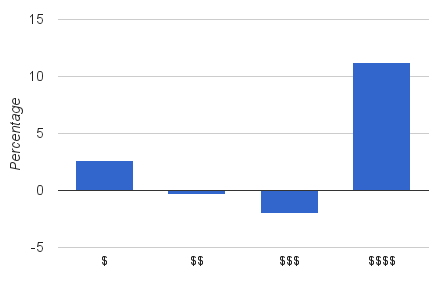
\includegraphics[width=.5\textwidth]{fig/ndcg-vs-price.png}
  \caption{Percentage improvement of \emph{SolocoRank} NDCG values in a particular
  price bracket in comparison to the overall NDCG value. NDCG values are
  higher for the highest-tier and lowest-tier of prices.}
  \label{fig:ndcg-vs-price}
\end{figure}

As is the case with most machine learning applications,
\emph{SolocoRank} is highly dependent on how features are represented
and various parameters that dictate how the model is composed.
For example, we noticed early on that \emph{SolocoRank} performs
substantially better for high-priced restaurants.
Figure \ref{fig:ndcg-vs-price} shows the average NDCG values,
when test sets are separated by price point.

We can attribute this to two factors. 
First of all, our training data highly depends on which restaurants
that Zagat chooses to rate.
At the moment, this decision is something we do not have any insight into.
Second, the consumer behavior is highly complex, dynamic, and in many times hard to capture.
The act of checking in is a very new phenomenon and may not be as
prevalent in certain cities or in certain classes of society.

\begin{figure}[h]
  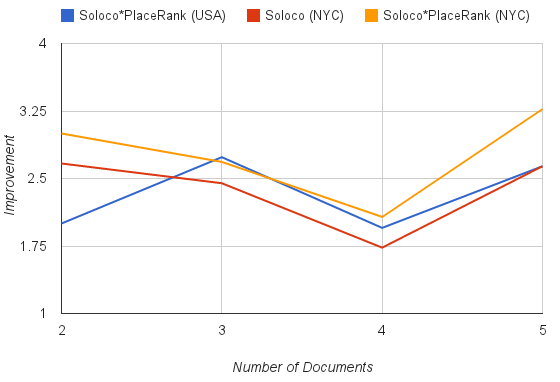
\includegraphics[width=.5\textwidth]{fig/localclassifier.png}
  \caption{Performance gains when training on only local data (New York City). 
  We count the number of test sets where the NDCG is higher for SolocoRank, compared
  to user review scores.
  Local classifiers perform 2-3 times better than a general model trained on all
  US Zagat data.}
  \label{fig:localclassifier}
\end{figure}

In the case of location, we wanted to evaluate the performance of \emph{SolocoRank},
trained only on local data. In other words, we removed location as a feature
and trained a classifier only on Zagat-rated restaurants in the New York City area.
Figure \ref{fig:localclassifier} shows the result of this evaluation.
We plot the improvement in the number of test sets where the NDCG was higher over \emph{SolocoRank}.
When \emph{SolocoRank} was only trained on local NYC places, 
there was a 2-3 times improvement over a general model trained on
all data in the US.

While it would be nice to have one general classifier,
it may be advantageous to train separate localized classifiers for each 
major metropolitan area due to the complex nature of location.
Further evaluation would need to be performed to argue whether
this is true of any other feature, such as price bracket.
However, this decision must be made with care, as the space of
classifiers quickly explode with more localization.

\subsection{Additional Data Sources}
In all of our evaluations, we only use features based on counts and
discrete assigned scores.
However, research has shown that free-form text may contain
valuable information that acts as strong signals for recommendations \cite{ganu2009}.
Future work ought to use advanced sentiment analysis techniques on reviews
to generate more features and strengthen the model.

Furthermore, as users are increasingly relying on online mapping services,
we can use a variety of new signals from these services.
For example, we use click-through data or even count the number of times
a user gets directions to a particular establishment.

\subsection{Alternative Labels}
In this paper, we make the assumption that Zagat is ultimately the ground truth
in quality distinctions.
This allows us to evaluate our ranker on relevance scores from external raters.
However, Zagat scores could instead be encoded as features.

Because \emph{SolocoRank} is a general learn-to-rank architecture,
any other score could be used as the training labels.
This could include other editorial review services, or even the rater's
relevance scores directly.
It is an open question, which signal most accurately reflects 
general consumer opinion on quality.

